\chapter{Simulating growth curves for diauxic shift}\label{chap:sim}
\section{Introduction}
Growth as a biological process is influenced by both metabolic and regulatory effects. 
We propose a model, composed of two networks: a gene regulatory network and a metabolic network. These networks interact with eachother 
predicting growth curves given a gene knockout experiment. We will begin by explaining the two types of networks and
how they are modelled individually before explaining the interaction between the two networks.
\section{Gene Regulatory Network}
\subsection{Introduction}
A gene regulatory network(GRN) is a network of regulators, such as genes, gene complexes and metabolites that interact. These interactions are symbolized
with connections in the network and the network controls the gene expression levels. They play a role in the development and differentiation of organisms
as well as in response to environmental changes.
\subsection{Formal Description}
The gene regulatory network is modelled as a directed graph $G(V,E)$ with parameters associated to the vertices $V$ and edges $E$, respectively $\theta_v$ and $\theta_e$. 
Furthermore every vertex starts with an (known)
initial value $g_v[0]$ and additionally, an updating function $\mathbf{g_v}[t] = f_{update}(\mathbf{g_v}[t-1], \mathbf{exp};\boldsymbol{\theta_e}, \boldsymbol{\theta_v})$ maps
the vector of values of the vertices $\mathbf{g_v}[t-1]$ to their subsequent values $\mathbf{g_v}[t]$ for the next time step $t$ given a certain biological experiment $\mathbf{exp}$. 
By repeatedly applying the update function, we thus obtain a time series of values for every individual vertex. 
\subsection{Updating function}\label{sec:update}
In the previous section we discussed at a high level that there is some function mapping the values of vertices to their values at the next time step. 
We want to learn a function $f_{exp}$ that maps an experiment $\mathbf{exp}$ to a time series of node states or: $ f_{exp}: \mathbf{exp} \to \mathbb{R}^{N \times T}$ where $N$ is the amount of nodes in the network and $T$ the amount of
discrete timepoints for which the values have to be estimated and $\mathbf{exp}$ is a tuple corresponding to a biological experiment. To this purpose we first learn a function $f_{update\_gene}$ for each node $i$ in the network that 
estimates the value of the next time step given the values of the current time.
From previous studies\cite{geistlinger2013comprehensive} there is already information available about the structural aspects of the GRN for the diauxic shift. 
Based on this we defined the regression task as following: 
\begin{equation}
 g_v[t+1] = f_{update\_gene}(Pa(g_v[t]) \cup g_v[t])
\end{equation}
where $g_v$ are genes, $t$ is time, $Pa(\cdot)$ indicates the parents of a gene.
We assume that the level of a gene at a certain time is dependent on the the influential genes from \cite{geistlinger2013comprehensive} and itself at the previous time. We also discretize time for this purpose and assume
gene level updates are done in a synchronous manner.
\subsection{Modelling interventional experiments}
Up till now, we only defined how to map gene levels from one time step to gene levels of the subsequent step. However we are interested in predicting the output for biological knockout experiments. 
To accomplish this these biological experiments are modelled as operations that can occur on vertices of the networks in the simulator. The first operation, also shown in figure \ref{fig:explanation_knockout}, performs a knockout of a vertex. 
In a graph based context this corresponds to removing all edges, both incoming and outgoing, from the vertex that was knocked out\cite{ud2015optimal} and this new configuration is then kept throughout the simulation. It is important to note that
 in a biological context this is a simplification of what is actually occurring as it cannot be guaranteed that the gene will not influence other genes (albeit with a small effect).
\begin{figure}
    \centering
    \begin{subfigure}[b]{0.3\textwidth}
        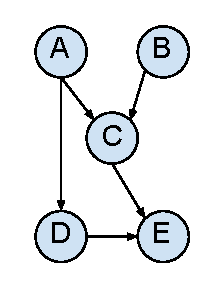
\includegraphics[width=\textwidth]{images/Graph_to_explain_gene_knockout.pdf}
        \caption{ Toy gene regulatory network for wild type i.e. without any knockouts }
        \label{fig:pre_knockout}
    \end{subfigure}
    \begin{subfigure}[b]{0.3\textwidth}
        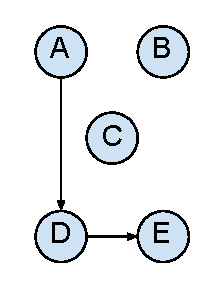
\includegraphics[width=\textwidth]{images/Graph_2_to_explain_gene_knockout.pdf}
        \caption{Same toy gene regulatory network, but where gene C is knocked out}
        \label{fig:with_knockout}
    \end{subfigure}
    \caption{ As an example of a gene knockout experiment, consider the toy gene regulatory network in \ref{fig:pre_knockout}. When we knock out vertex C, it corresponds to cutting all incident and outgoing edges of C. }
    \label{fig:explanation_knockout}
\end{figure}
An additional operation is adjusting the initial values based on the values for the input. In contrast with the previous operation, these values are not kept stationary in subsequent timesteps of a simulation, but they will be 
updated as specified in section \ref{sec:update}.
\subsection{Initial values for the network}
For the initial values of the vertices, we took two different approaches. For the first approach we took two datasets\cite{brauer2008coordination,brauer2005homeostatic} that investigate gene expressions before, during and after
the diauxic shift and used the normalized starting values as the initial values. The second approach consisted of a probabilistic/statistical approach. We  extracted the gene expression levels
for yeast under many different environments from \cite{faith2008many}. Based on these values we estimated the marginal distributions of the genes by fitting them to different continuous probability distributions and selecting the fit that has the lowest
Bayesian information criterion\footnote{$BIC = -2 \ln L + k \ln(n)$ where $L$ is the maximized value of the likelihood,
$n$ is the number of data points and $k$ is the number of free parameters.} value. Based on previous studies 
regarding the continuous distributions of genes \cite{NEEDED} only the Weibull, Gaussian and Gamma distributions were
considered. 
\section{Metabolic Network}
\subsection{Introduction}
A metabolic network consists of all cellular biochemical reactions catalyzed by enzymes as together they form interconnected metabolic pathways
and as such a network. The vertices are called metabolites, which comprises all intermediates or products that in the metabolism of an organism.
\subsection{Dynamic flux balance analysis}
``In flux balance analysis, one constrains the metabolic network by the balance of metabolic fluxes around metabolites. 
When the metabolic network is operating in a steady state, the mass balance is described by a set of linear equations.''
\cite{mahadevan2002dynamic}
When the batch time is divided into several time intervals and the optimization problem is solved at the beginning of 
each time interval, one can get a dynamic solution for the metabolic fluxes. The results are then integrated over the intervals.
\section{Interaction between GRN and Metabolic Network}\label{sec:fba}
Thus far the GRN and metabolic network have only been discussed separately from eachother, but it's possible to combine
them. The GRN contains several nodes that are actually metabolites and therefore values obtained by the flux balance analysis
can be fed to the GRN. Additionally, the metabolic network contains information about what genes are influencing what
chemical reactions. Dependent on the value of those genes, the optimization problem can be redefined by adapting the 
relevant maximal fluxes. 
To map the values of the network from the ranges $[-1,1]$ to $[0,1]$, we feed the gene values to a parametrized logistic function.
% Figure \ref{fig:simulator} shows at a high level how the simulator is composed and what the inputs
and outputs of the systems are. Additionally, pseudocode of the simulator is available at \ref{alg:combi_simulator}.
\begin{figure}	
    \centering
    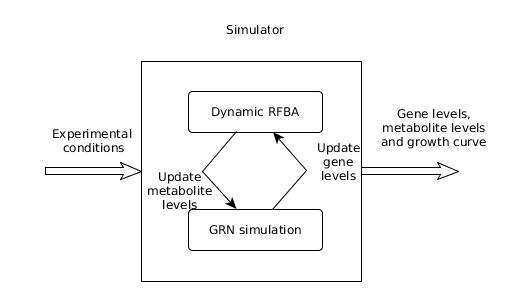
\includegraphics[width=0.4\textwidth]{images/simulator.png}
    \caption{ Illustration of the inputs, outputs, networks and dynamics of the simulator. }
    \label{fig:simulator}
\end{figure}
\begin{algorithmic}\label{alg:combi_simulator}
  \Function{ simulation }{ experiment, initialVertexValues, modelParameters } 
  \Require experiment, initialVertexValues, modelParameters
  \State metabolicModel, geneRegulatoryModel $\leftarrow$ initialize\_networks( modelParameters )
  \State metaboliteValues[0] $\leftarrow$ initializeVertices(metabolicModel, geneRegulatoryModel, initialVertexValues)
  \State adaptWithExperiment(metabolicModel, geneRegulatoryModel, experiment)
  \For{ time in 0:experiment.totalTime }
  \State geneValues[time+1] $\leftarrow$ grnSimulation( geneRegulatoryModel, metaboliteValues[time] )
  \State metaboliteValues[time + 1], growth[time + 1] $\leftarrow$ metabolicSmulation( metabolicModel, geneValues[time+1] )
  \EndFor \\
  \Return growth, geneValues, metaboliteValues
  
  \EndFunction 
\end{algorithmic} 

\section{Probabilistic Estimates}
As typically, there are different sources contributing to uncertainty. The simulator was extended to allow to express different aspects of this uncertainty: initial levels of vertices, model parameters, experimental values.
Currently we only allow specification by means of a (continuous) uniform, Gaussian or Beta distribution, however we can easily extend this to other, both continuous as discrete, distributions.	
Additionally, a combination of deterministic and probabilistic information is still possible: for instance if we are certain that knocking out a gene completely disables the corresponding vertex, the vertex can be completely cut out. However if
there could be a small non-zero value associated with that vertex, it might be more suitable to model it by means of a probability density function. The 
\section{Results}
\subsection{Results of estimates for gene regulatory network}
\subsubsection{Data}
Available datasets can typically be divided in two types: time-course experiments to observe changes in expression levels over time and perturbation experiments to observe effects of a change or treatment on a cell. Since our interest with 
regard to the gene regulatory network lies on the temporal behaviour of gene regulation i.e. the dynamical behaviour, we only selected timeseries datasets from SGD\footnote{http://www.yeastgenome.org/download-data/expression}. We did not 
limit ourselves to datasets solely concerning diauxic shift as we assume that the genetic influences can be averaged over the different conditions. 
This resulted in the following subset: \cite{brauer2005homeostatic,spellman1998comprehensive,cho1998genome,derisi1997exploring,lee2000arrest,carmel2001role}.
Prior to regression tasks, the datasets were normalized (independently from eachother) such that all expression values are contained in the interval $[-1,1]$.%http://libsleipnir.bitbucket.org/Normalizer.html
We obtain appropriate datasets by choosing a $t_{defined}$ and only selecting those datapoints for which we have data of $\Delta t = t_{defined}$. As the datasets are very diverse in their timescales, this results less available data per reaction. These time 
difference are expected to have a significant effect on the output. This resulted in datasets for which the summary can be found in table \ref{tab:summary_time_datasets}.
\begin{table}[htb]
	\centering
   % \resizebox{0.3\textwidth}{!}
   % {
    \begin{tabular}{llll}
    \hline
$\Delta t$(min)&Min&Max&Mean\\
\hline
10&37&94&82.14\\
15&58&111&101.91\\
20&7&53&44.42\\
30&86&170&153.04\\
60&70&136&121.32\\
120&22&52&46.68\\
180&11&31&27.95\\
    \hline
    \end{tabular}
  %  }
    \caption{ Summary of amount of datapoints available per reaction for different time differences. Reported are the minimum amount of data for a reaction, the maximum amount and the average amount. }
	\label{tab:summary_time_datasets}

\end{table}
\subsection{Results of estimates for gene regulatory network}
We trained both a linear support vector regressor and one with an RBF kernel\footnote{with hyperparameter values $C \in \{ 2^k \forall k \in [-10,15[ : k \in \naturalspace \}$ and 
$\epsilon = \{0,0.01,0.05,0.1,0.15,0.2\}$ and L1 loss function} as specified in section \ref{sec:update}.
The results are summarized in table \ref{tab:summary_v_1}, which shows different qualitative measures for the different regressors and for the different time discretizations, but for more clarity only the best time discretizations are shown.
After the hyperparameters were determined by 10-fold crossvalidation, the regressor was retrained with the whole training set. Reported results are on a separate testset, divided in two 80\%-20\% disjoint sets (respectively training and test set).
The linear version is better than the RBF SVR, suggesting that a linear approximation is not necessarily a bad approximation. As a starting network for further optimization, we will therefore use the parameters obtained from the linear support vector
regressor with the discretization of 30 minutes.
Subsequent gene levels are calculated by the following formula:

\begin{equation}\label{eq:gene_update}
 g_v[t+1] = \sum_{j : g_j \in Pa(g_v) \cup \{g_i\} } \theta_{e,(i,j)}g_j[t] + \theta_{v,i}
\end{equation}
\begin{landscape}
\begin{longtable}[htb]{|l|l|l|rrrrr|}

    \hline
Learner& $\Delta$t&Type&Min&Max&Mean&Stdev&Median\\ \hline
\multirow{14}{*}{SVR\textsubscript{Linear}}&\multirow{4}{*}
{20 min}
&MAE&0.0159&0.2879&0.0867&0.0016&0.0779\\
&&MSE&0.0003&0.1612&0.0158&0.0003&0.0099\\
&&MedAE&0.0139&0.2435&0.0687&0.0014&0.061\\
&&$R^2$&-20.5604&0.9725&0.2555&2.8958&0.6092\\
\cline{2-8}
&\multirow{4}{*}{30 min}
&MAE&0.0378&0.4082&0.0879&0.0012&0.0823\\
&&MSE&0.0025&0.2411&0.0161&0.0003&0.0121\\
&&MedAE&0.0217&0.3196&0.0683&0.0009&0.0627\\
&&$R^2$&-1.6544&0.8871&0.4311&0.1062&0.4944\\

\cline{2-8}
&\multirow{4}{*}{60 min}
&MAE&0.027&0.2427&0.0971&0.0012&0.091\\
&&MSE&0.0018&0.1156&0.0198&0.0003&0.0154\\
&&MedAE&0.0217&0.1986&0.0715&0.0009&0.0656\\
&&$R^2$&-1.1329&0.8619&0.3672&0.0997&0.4185\\
\hline
\multirow{14}{*}{SVR\textsubscript{RBF}}&\multirow{4}{*}{20 min}
&MAE&0.0157&0.241&0.0895&0.0014&0.0827\\
&&MSE&0.0004&0.0907&0.0147&0.0002&0.0098\\
&&MedAE&0.0058&0.2366&0.0761&0.0012&0.0716\\
&&$R^2$&-129334.1088&0.9561&-397.5627&51468962.4212&0.6484\\
\cline{2-8}
&\multirow{4}{*}{30 min}
&MAE&0.04&0.2983&0.0851&0.001&0.0786\\
&&MSE&0.003&0.1682&0.0145&0.0002&0.0106\\
&&MedAE&0.0235&0.2722&0.0675&0.0008&0.0632\\
&&$R^2$&-1.1632&0.8885&0.4661&0.0769&0.5155\\
\cline{2-8}
&\multirow{4}{*}{60 min}
&MAE&0.0459&0.262&0.0949&0.0009&0.0897\\
&&MSE&0.0033&0.1309&0.0178&0.0002&0.0143\\
&&MedAE&0.0272&0.2283&0.0737&0.0008&0.0687\\
&&$R^2$&-3.792&0.8471&0.3839&0.1352&0.4388\\
\hline
    \caption{Summary of the results for the learned regressors for the updating function as described in section \ref{sec:update} }
	\label{tab:summary_v_1}
\footnotesize
\end{longtable}
\end{landscape}


\subsection{ Results of combined model }
